\section{表面吉布斯自由能}


\begin{frame}
    \frametitle{常见的表面}
    \begin{figure}[htpb]
        \centering
        \setcounter{subfigure}{0}
        \subfloat[气液、液液界面]{
\includegraphics[height=2.5cm]{气液}}\quad
        \subfloat[气固界面]{
\includegraphics[height=2.5cm]{气固}}\\
        \subfloat[液固界面]{
\includegraphics[height=2.4cm]{液固}}\quad
        \subfloat[固固界面]{
\includegraphics[height=2.4cm]{固固}}
    \end{figure}
\end{frame}


\begin{frame}
    \frametitle{界面现象的本质}
    表面层显示出一些独特性质，如表面张力、表面吸附、毛细现象、过饱和状态等。其本质是因为表面层分子与内部分子相比所处的环境不同。

    体相内部分子所受四周邻近相同分子的作用力是对称的，各个方向的力彼此抵销；但是处在界面层的分子，一方面受到体相内相同物质分子的作用，另一方面受到性质不同的另一相中物质分子的作用，其作用力未必能相互抵销，因此，界面层会显示出一些独特的性质。

    \begin{figure}[htpb]
        \centering
        
\includegraphics[width=.5\linewidth]{fig8.1}
    \end{figure}
\end{frame}


\begin{frame}
    \frametitle{比表面}

    表面现象显著的体系常是高度分散的体系，如粉末状或多孔状物质、水中的气泡、油滴等。衡量多相分散体系的分散程度通常用比表面(specific surface)表示
    \[
        S_0 = \frac{A}{V} \quad \text{或} \quad S_0 = \frac{A}{m}
    \]
    式中$A$为体积为$V$或质量为$m$的物质所具有的总表面积。
    
    比表面$S_0$就是单位体积或单位质量的物质所具有的表面积，单位是$m^{-1}$或\si{m^2.kg^{-1}}。
    
    当将固体颗粒或液滴的尺寸逐渐降低时，比表面$S_0$的数值将随之迅速增加。

\end{frame}


\begin{frame}[t]{}
    \begin{example}
        一滴体积$V = \SI{e-6}{m^3}$的水滴，当被分散为半径分别是$r_1 = \SI{e-3}{m}$，$r_2 = \SI{e-4}{m}$，$r_3 = \SI{e-6}{m}$和$r_4 = \SI{e-8}{m}$的小液滴时，分散成的水滴总数、比表面和总表面积各为多少？
    \end{example}\pause
    \begin{table}[]
        \begin{tabular}{cccc}
        \hline
        水滴半径/m & 液滴数目 & 比表面$S_0/\mathrm{m}^{-1}$ & 总表面积$A/\mathrm{m}^{2}$ \\ \hline
        $6.2\times 10^{-3}$ & 1 & $4.8\times 10^2$ & $4.8\times 10^{-4}$ \\
        $10^{-3}$ & $2.4\times 10^2$ & $3\times 10^3$ & $3\times 10^{-3}$ \\
        $10^{-4}$ & $2.4\times 10^5$ & $3\times 10^4$ & $3\times 10^{-2}$ \\
        $10^{-6}$ & $2.4\times 10^{11}$ & $3\times 10^6$ & 3 \\
        $10^{-8}$ & $2.4\times 10^{17}$ & $3\times 10^8$ & $3\times 10^2$ \\ \hline
        \end{tabular}
        \end{table}

\end{frame}


\begin{frame}
    \frametitle{比表面自由能}

        \begin{minipage}{0.48\linewidth}
            表面层分子与体相内分子所处环境不同。表面层分子主要受到指向液体内部的拉力，使得表层分子有向液体内部迁移、液体表面积自动收缩的趋势。
        \end{minipage}\hfill
        \begin{minipage}{0.48\linewidth}
            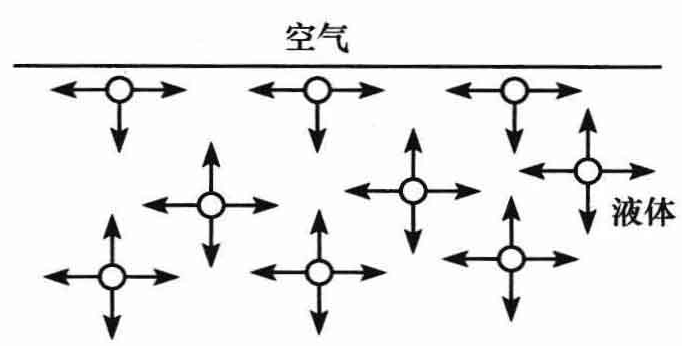
\includegraphics[width=\linewidth]{figures/fig8.1.png}
        \end{minipage}

        \highlight{表面功}：如果要扩大液体表面，即把一些分子从液相内部移到表面上，就必须克服液体内部分子之间的吸引力而对体系做功，此功称为表面功。

        定温、定压，组成恒定时，
        \[
            \delta W' = \sigma\dif A
        \]
        表面功$\delta W'$为可逆非体积功，$\sigma$为比例常数。
\end{frame}


\begin{frame}
    \frametitle{比表面自由能}

    定温定压下体系可逆地扩展表面所得到的表面功应等于吉布斯自由能的增加量，$\dif G = \delta W'$。
    \[
        \dif G = \sigma\dif A \qquad \text{或} \qquad \sigma = \left(\frac{\partial G}{\partial A}\right)_{T,p,n}
    \]
    $\sigma$的物理意义是当$T$、$p$及组成恒定时，增加单位表面积所引起的吉布斯自由能的增量。
    
    $\sigma$称为比表面自由能，单位\si{J.m^{-2}}。
    
    当可逆地形成新表面时，环境所做的表面功转化为表面层分子的吉布斯自由能。表层分子因此比体相内分子具有更高的能量，$\sigma$也称为表面过剩吉布斯自由能，简称表面能。

\end{frame}


\begin{frame}
    \frametitle{表面张力}

    表面现象还可以从力的角度描述。气-液界面两边物质不同，其密度也不同，故液体表面存在使其面积减小的力，称为表面张力（或界面张力）。其物理意义是在与液面相切方向上垂直作用于单位长度线段上的收缩力。表面张力也用符号$\sigma$表示，单位为\si{N.m^{-1}}。表面张力与比表面自由能在数值上完全相等，并有相同的量纲，但物理意义不同，是从不同角度反映体系的表面特征。

    表面张力的大小与物质种类、共存另一相的性质以及温度和压力等因素有关。
    
    测量表面张力的方法有：
    \begin{enumerate}
      \item 吊板法
      \item 滴重法
      \item 最大泡压法
      \item 毛细管上升法
    \end{enumerate}

\end{frame}